\documentclass[submit]{harvardml}

% You don't need to change these.
\course{CS181-S19}
\assignment{Assignment \#2}
\duedate{11:59pm Mar 1st, 2019} % FDV: Adjust to correct date

\usepackage[OT1]{fontenc}
\usepackage[colorlinks,citecolor=blue,urlcolor=blue]{hyperref}
\usepackage[pdftex]{graphicx}
\usepackage{subfig}
\usepackage{fullpage}
\usepackage{amsmath}
\usepackage{amssymb}
\usepackage{color}
\usepackage{soul}
\usepackage{todonotes}
\usepackage{listings}
\usepackage{common}
\usepackage{bm}
\graphicspath{ {./images/} }


\usepackage[mmddyyyy,hhmmss]{datetime}

\definecolor{verbgray}{gray}{0.9}

\lstnewenvironment{csv}{%
  \lstset{backgroundcolor=\color{verbgray},
  frame=single,
  framerule=0pt,
  basicstyle=\ttfamily,
  columns=fullflexible}}{}

\begin{document}


{
  \begin{center}
{\Large Homework 2: Bayesian Methods and Multiclass Classification}\\
\end{center}
}
\subsection*{Introduction}

% FDV: Make sure that the readings are relevant to the problems and
% that the descriptions match.

This homework is about Bayesian methods and multiclass
classification. In lecture we have primarily focused on binary
classifiers trained to discriminate between two classes. In multiclass
classification, we discriminate between three or more classes. We
encourage you to first read the Bishop textbook coverage of these
topic, particularly: Section 4.2 (Probabilistic Generative Models),
Section 4.3 (Probabilistic Discriminative Models).

As usual, we imagine that we have the input matrix $\boldX \in
\reals^{n \times m}$ (or perhaps they have been mapped to some basis
$\bm{\Phi}$, without loss of generality) but our outputs are now
``one-hot coded''.  What that means is that, if there are~$c$ output
classes, then rather than representing the output label $y$ as an
integer~${1,2,\ldots,c}$, we represent $\boldy$ as a binary vector of
length~$c$. These vectors are zero in each component except for the
one corresponding to the correct label, and that entry has a one.  So,
if there are 7 classes and a particular datum has label 3, then the
target vector would be~${C_3 = [0,0,1,0,0,0,0]}$.  If there are $c$
classes, the set of possible outputs is $\{C_1 \ldots C_c \} =
\{C_k\}_{k=1}^c$.  Throughout the assignment we will assume that
output $\boldy \in \{C_k\}_{k=1}^c$.\\

The problem set has three problems:
\begin{enumerate}
\item In the first problem, you will explore the properties of
  Bayesian estimation methods for the Bernoulli model.
%
\item In the second problem, you will dive into matrix algebra and the
  methods behind generative multiclass classifications. You will
  extend the discrete classifiers that we see in lecture to a Gaussian
  model.
%
\item Finally, in the third problem, you will implement logistic
  regression as well as a generative classifier from close to scratch.
%
\end{enumerate}

\newpage
\begin{problem}[Bayesian Methods, 10 pts]

  This question helps to build your understanding of the
  maximum-likelihood estimation (MLE) vs. maximum a posterior
  estimator (MAP) vs. a posterior predictive.\\

  % FDV: Make sure that the lecture reference is accurate below.
  First consider the Beta-Bernoulli model (and see lecture 5.)  Let
  $\theta$ be the probability that a coin comes up heads.  Consider a
  prior $\theta\sim Beta(2,2)$, and data $D= 0, 0, 1, 1, 0, 0, 0, 0,
  1, 0, 1, 1, 1, 0, 1, 0$.

%
\begin{enumerate}

\item 
We are interested in seeing how $\theta$, the probability that a coin comes up heads, changes as we get more data.
 Write down the expressions for: 
 \begin{enumerate}
     \item the maximum likelihood estimate of $\theta$
     \item the MAP estimate of $\theta$
     \item the posterior predictive estimate of $\theta$ based on $P(X = 1 | D)$, where $X$ is a new flip and $D$ is all the data you currently have.
 \end{enumerate} 
 Notice in the case of the Beta-Bernoulli model, the posterior predictive can also be represented as a point estimate of $\theta$, which is not always the case! 
 
 Plot each of three different estimates after each
  additional sample.  You can consider making a single plot with
  flips on the x-axis and three lines showing your guess for the
  probability of heads after each flip for each estimator.

%
\item Interpret the differences you see between the three different
estimators.
% 
\item Plot the posterior distribution (prior for 0 examples) on $\theta$ after 0, 4, 8, 12 and 16 examples. (Using whatever tools you like.)  You may make separate plots for each or overlay all the plots to visualize how the posterior on $\theta$ changes.
%

% FDV: The two problems below are new and will need solutions written out.
\item Compute the marginal likelihood of the training data $p(D)$.
  Hint: Notice that the required integral looks like an unnormalized
  Beta distribution, and take advantage of the fact that integrating
  over a normalized Beta distribution is equal to 1.
  %
\item Now consider an alternate model in which our prior over the coin
  is that it likely comes up heads or likely comes up tails, that is
  $\theta \sim \frac{1}{2}( Beta(10,1) + Beta(1,10) )$.  Compute the marginal
  likelihood for this model.  Which of the two models has a higher
  marginal likelihood?
\end{enumerate}
 \end{problem}
\subsection*{Solution}

\begin{enumerate}
    \item 
    \begin{enumerate}
        \item[(a)] The likelihood function of $\theta$, $L(\theta ;D)$, where $D$ represents all the data, is equal to $P(D ; \theta)$. Since we have a Bernoulli model and $\theta$ is the probability that a coin comes up heads, we have
        
        $$L(\theta ;D) = P(D ; \theta) = \theta^H(1-\theta)^T$$
        
        where $H$ is the total number of heads and $T$ is the total number of tails. We observed $H, T = 7, 9$. I got this likelihood by multiplying the probability of each data point occurring. Now, to find the MLE, we will maximize this w.r.t. $\theta$. Take the log first to simplify the calculation (without changing the maximum since log is monotonically increasing).
        
        $$\ln L(\theta ;D) = l(\theta ;D)= H\ln\theta + T\ln(1-\theta)$$
        
        $$ \implies l'(\theta ;D)= \frac{H}{\theta} - \frac{T}{1-\theta} = 0$$
        
        $$ \hat{\theta}_{MLE} = \frac{H}{H+T}$$
        
        This says that the MLE of $\theta$ is the number of heads in the data divided by the total number of flips. With out observed data, this is
        
        $$ \boxed{\hat{\theta}_{MLE} = \frac{7}{16}}$$
        
        \item[(b)] The MAP estimate of $\theta$ is the maximum of the likelihood of $\theta$ multiplied by the prior of $\theta$. Since we have a $\textrm{Beta}(2,2)$, prior, this is
        
        $$ P(D ; \theta)P(\theta) \propto \theta^H(1-\theta)^T \theta^1(1-\theta)^1 $$
        
        where I have dropped the normalizing constant of the prior since this will not affect the maximum of this value. This simplifies to 
        
        $$ P(D ; \theta)P(\theta) \propto \theta^{H+1}(1-\theta)^{T+1}$$
        
        Now, taking the log and maximizing w.r.t. $\theta$ yields
        
        $$\frac{H+1}{\theta} - \frac{T+1}{1-\theta} = 0$$
        
        $$ \implies \hat{\theta}_{MAP} = \frac{H + 1}{H + T + 2}$$
        
        In words, this says that the MAP estimate of $\theta$ is 1 plus the number of heads divided by the quantity, 2 plus the total number of flips. With our numbers this becomes
        
        $$ \boxed{\hat{\theta}_{MAP} = \frac{8}{18} = \frac{4}{9}}$$
        
        
        \item[(c)] Lastly, the posterior predictive estimate will be the expectation of the posterior distribution of $\theta$. By the properties of the beta distribution (beta-binomial conjugacy), the posterior will also be beta. Specifically, it will be $\textrm{Beta}(2+H, 2+T)$. This outcome was discussed in class and is also proved on page 354 of the Stat 110 textbook. Thus, the posterior predictive estimate will be the expectation of $\textrm{Beta}(2+H, 2+T)$. This is
        
        $$\hat{\theta}_{PP} = \frac{H+2}{H+T+4}$$
        
        In words, this says that the posterior predictive estimate of $\theta$ is 2 plus the number of heads divided by the quantity, 4 plus the total number of flips. With our numbers this becomes
        
        $$ \boxed{\hat{\theta}_{PP} = \frac{9}{20}}$$
        
    \end{enumerate}
    
    Below, I have plotted each of these three estimates after each additional sample. 
    
    \begin{center}
        \includegraphics[scale = 0.6]{1.png}
    \end{center}
    
    \item First, note that the posterior predictive estimate (the posterior expectation) and the MAP (the posterior mode) both depend on the choice of prior, and this is why they both start close to 0.5 since our prior distribution has a mean and mode of 0.5. In contrast, the MLE is simply the sample mean, so it starts out at 0. Since we never have a greater proportion of heads then tails in our data, the posterior distribution ($\textrm{Beta}(2+H, 2+T)$ as found in 1c) will always have a smaller first parameter than second parameter. When $a<b$ for $\textrm{Beta}(a,b)$, the beta has a right skew, so its mean is greater than its mode. Hence, this is why the PPE is always greater than the MAP throughout our experiment.
    
    Lastly, note that with enough trials, all of the estimates start to come to the same value, and the choice of the prior becomes less influential.
    
    \item
    
    Below is a plot of the posterior distribution after $D$ samples (the prior distribution when $D= 0$).
    
    \begin{center}
        \includegraphics[scale = 0.7]{13.png}
    \end{center}

As seen, the distribution starts off as our prior, a $\textrm{Beta}(2,2)$. Then the mode of the distribution moves leftward (while the mean also moves leftward but lags because of the skew) because there were many tails. Eventually, the the mode later moves back towards the center because the total number of heads (7) approaches the total number of tails (9). Fortunately, because of the properties of the beta distribution, all of these posterior distributions are still betas.

\item We would like to calculate $P(D)$ and we have $P(D|\theta)$. So, by the law of total probability, we can use

$$ P(D) = \int_0^1 P(D|\theta)P(\theta)d\theta$$

where we are integrating over the total support of $\theta$. Plugging in $P(D|\theta)$, and remembering that $\theta \sim \textrm{Beta}(2,2)$ this becomes

$$ P(D) = \int_0^1 \theta^H(1-\theta)^T \frac{\theta^1 (1-\theta)^1}{\beta(2,2)} d\theta = \frac{1}{\beta (2,2)}\int_0^1 \theta^{H+1}(1-\theta)^{T+1}  d\theta$$ 

$$ \implies P(D) = \frac{\beta(H+2, T+2)}{\beta (2,2)}\int_0^1 \frac{\theta^{H+1}(1-\theta)^{T+1}}{\beta(H+2, T+2)}  d\theta = \frac{\beta(H+2, T+2)}{\beta (2,2)}$$

Since this terms in the integral are a valid beta pdf. With our specific data, this becomes 

$$\boxed{P(D) = \frac{\beta(9, 11)}{\beta (2,2)} = 7.216 \times 10^{-6}}$$

\item
With this new model, we have that the marginal likelihood is now 

$$ P(D) = \int_0^1 P(D|\theta)P(\theta)d\theta = \frac{1}{2}\int_0^1 \theta^H(1-\theta)^T \frac{\theta^9 (1-\theta)^0}{\beta(10,1)} d\theta + \frac{1}{2}\int_0^1 \theta^H(1-\theta)^T \frac{\theta^0 (1-\theta)^9}{\beta(1,10)} d\theta$$

$$= \frac{1}{2} \frac{\beta(H+10,T+1)}{\beta(10,1)}\int_0^1 \frac{\theta^{H+9}(1-\theta)^T}{\beta(H+10,T+1)} d\theta + \frac{1}{2} \frac{\beta(H+1,T+10)}{\beta(1,10)}\int_0^1 \frac{\theta^H(1-\theta)^T}{\beta(H+1,T+10)}  d\theta$$

Again, realizing that these integrands are valid beta pdf's, this becomes

$$ P(D) = \frac{1}{2} [\frac{\beta(H+10,T+1)}{\beta(10,1)} + \frac{\beta(H+1,T+10)}{\beta(1,10)}] $$

Plugging in our actual data, this is

$$ \boxed{P(D) = \frac{1}{2} [\frac{\beta(17,10)}{\beta(10,1)} + \frac{\beta(8,19)}{\beta(1,10)}] = 4.942 \times 10^{-7}}$$

This model yields a smaller marginal likelihood, meaning our previous choice of prior is more likely to be accurate. Indeed, the data did not have a high number of heads and low number of tails (or vice versa), so it makes sense that this prior gave a smaller marginal likelihood.

\end{enumerate}


% FDV: The problem below is the same as last year, just check for clarity.
%%%%%%%%%%%%%%%%%%%%%%%%%%%%%%%%%%%%%%%%%%%%%
% Problem 2
%%%%%%%%%%%%%%%%%%%%%%%%%%%%%%%%%%%%%%%%%%%%%
\begin{problem}[Return of matrix calculus, 10pts]
  Consider now a generative $c$-class model.  We adopt class prior
  $p(\boldy = C_k; \bpi) = \pi_k$ for all $k \in \{1, \ldots, c\}$
(where $\pi_k$ is a parameter of the prior).
%
%that define the prior.
Let  $p(\boldx|\boldy=C_k)$ denote
the class-conditional density of features $\boldx$ (in this
case for class $C_k$). Consider the data set $D = \{(\boldx_i,
\boldy_i)\}_{i=1}^n$ where as above $\boldy_i \in \{C_k\}_{k=1}^c$ is
encoded as a one-hot target vector.
%
\begin{enumerate}
  \item Write out the negated log-likelihood of the data set,
    $-\ln p(D ; \bpi)$.
%
  \item Since the prior forms a distribution, it has the constraint that
    $\sum_{k=1}^c\pi_k - 1 = 0$.  Using the hint on
Lagrange multipliers below, give the
    expression for the maximum-likelihood estimator for the prior
    class-membership probabilities, i.e.
    $\hat \pi_k.$
    Make sure to write out the intermediary equation you need
    to solve to obtain this estimator. Double-check your answer: the final
    result should be very intuitive!
\end{enumerate}
    For the remaining questions, let the
    class-conditional probabilities be Gaussian distributions with
the same covariance matrix
    $$p(\boldx | \boldy = C_k) = \mathcal{N}(\boldx |  \bmu_k, \bSigma), \text{\ for\ }k \in \{1,\ldots, c\}$$
%
and different means $\bmu_k$ for each class.
%
    \begin{enumerate}
  \item[3.] Derive the gradient of the negative log-likelihood with respect to vector $\bmu_k$.
    Write the expression in matrix form as a function of the variables defined
    throughout this exercise. Simplify as much as possible for full credit.
  \item[4.] Derive the maximum-likelihood estimator for vector $\bmu_k$. Once
    again, your final answer should seem intuitive.
  \item[5.] Derive the gradient for the negative log-likelihood with respect to the
    covariance matrix $\bSigma$ (i.e., looking
to find an MLE for the covariance).
Since you are differentiating with respect to a
    \emph{matrix}, the resulting expression should be a matrix!
%
  \item[6.] Derive the maximum likelihood estimator of the covariance matrix.
\end{enumerate}
\paragraph{Hint: Lagrange Multipliers.} Lagrange Multipliers are a method for
optimizing a function $f$ with respect to an
equality constraint, i.e.
\[\min_{\boldx} f(\boldx)\ \text{s.t.}\ g(\boldx) = 0.\]
This can be turned into an unconstrained problem by introducing a
Lagrange multiplier $\lambda$ and constructing the Lagrangian function,
\[L(\boldx, \lambda) =  f(\boldx) + \lambda g(\boldx).\]
It can be shown that it is a necessary condition that the optimum
is a critical point of this new function. We can find this point by solving two equations:
\[\frac{\partial L(\boldx, \lambda)}{\partial  \boldx} = 0  \ \ \text{and}\  \  \frac{\partial L(\boldx, \lambda)}{\partial \lambda} = 0 \]
\paragraph{Cookbook formulas.} Here are some formulas you might want to consider
using to compute difficult gradients. You can use them  in the homework
without proof. If you are looking to hone your matrix calculus skills, try to
find different ways to prove these formulas yourself (will not be part of the
evaluation of this homework). In general, you can use any formula from the matrix cookbook,
as long as you cite it. We opt for the following common notation:
$\boldX^{-\top} := (\boldX^{\top})^{-1}$
\begin{align*}
  & \frac{\partial \bolda^\top \boldX^{-1} \boldb}{\partial \boldX} = - \boldX^{-\top} \bolda \boldb^\top \boldX^{-\top} \\
  & \frac{\partial \ln | \det (\boldX) |}{\partial \boldX} = \boldX^{-\top}
 \end{align*}
 \end{problem}
\subsection*{Solution}

\begin{enumerate}
    \item We have
    
    $$p(D;\pi) = \prod_{i=1}^n p(x_i ; \pi)$$
    
    By Law of Total Probability, we have
    
    $$p(D;\pi) = \prod_{i=1}^n \prod_{k=1}^c [p(x_i |y_i = C_k) p(y_i =C_k ; \pi)] ^{I_{y_i=C_k}} $$
    
    where I have added an indicator r.v. in the exponent which will be $1$ if $y_i=C_k$ and $0$ otherwise since we only wish to include this probability for our given $i$ and $k$ if $x_i$ has has class $C_k$. Note, in order for this to make sense, I am choosing to view $y_i$ as not being one-hot encoded. Alternatively, $C_k$ can be viewed as one hot encoded in this indicator. The point is that $I_{y_i=C_k}$ is only equal to 1 if the $i$'th data point label is equal to the label of the $k$'th class. Now, plugging in the given expression for $p(y_i =C_k ; \pi)$, we have
    
    $$p(D;\pi) = \prod_{i=1}^n \prod_{k=1}^c [p(x_i |y_i = C_k) \pi_k] ^{I_{y_i=C_k}} $$
    
    Taking the log and negating then yields 
    
    $$\boxed{- \ln p(D;\pi) = -\sum_{i=1}^n \sum_{k=1}^c [ \ln p(x_i |y_i = C_k) +\ln(\pi_k)] I_{y_i=C_k}} $$
    
    This is the negative log likelihood.
    \item Using the hint, I can write out the Lagrangian function
    
    $$ -\sum_{i=1}^n \sum_{k=1}^c [ \ln p(x_i |y_i = C_k) +\ln(\pi_k)] I_{y_i=C_k} + \lambda(\sum_{k=1}^c \pi_k -1) $$
    
    I would like to minimize this with respect to each $\pi_k$ for every $k$ and with respect to $\lambda$. This is the same as
    
    $$ \max_{\pi_k,\lambda} [\sum_{i=1}^n \sum_{k=1}^c [ \ln p(x_i |y_i = C_k) +\ln(\pi_k)] I_{y_i=C_k} - \lambda(\sum_{k=1}^c \pi_k -1)] $$
    
    Now I must take the derivatives. Note that the derivative of $p(x_i |y_i = C_k)$ w.r.t. $\pi_k$ is $0$ since this is a constant for given $\pi_k$. Also, $I_{y_i=C_k}$ can be treated as a constant since it is always either $0$ or $1$. So, this yields the $C + 1$ equations:
    
    $$ \textrm{w.r.t. $\lambda$: }\sum_{k=1}^c \pi_k -1 = 0 \implies \sum_{k=1}^c \pi_k =1 $$
    
    $$ \textrm{w.r.t. a specific $\pi_k$: } \sum_{i=1}^n \sum_{k=1}^c \frac{I_{y_i=C_k}}{\pi_k} -\lambda = 0 \implies \lambda=\sum_{i=1}^n \sum_{k=1}^c \frac{I_{y_i=C_k}}{\pi_k} = \frac{n_k}{\pi_k} $$
    
    where $n_k$ is the number of data points with class $k$. Combining these equations, we see that
    
    $$ \sum_{k=1}^c \pi_k =1 \implies \sum_{k=1}^c \frac{n_k}{\lambda} =1 \implies \lambda = \sum_{k=1}^c n_k \equiv n$$
    
    $$ \implies \boxed{\hat{\pi}_k = \frac{n_k}{\sum_{j=1}^c n_j} = \frac{n_k}{n}}  $$
    
    To ensure this is indeed a maximum, we can take the second derivatives, but this would involve $c+1$ derivatives and a high dimensional jacobian. So, instead, realize that the log likelihood is convex w.r.t $\pi_k$. Thus, we can conclude that we have indeed found a maximum of the likelihood (or a minimum of the negated log likelihood).
    
    Also, note that this has an intuitive result. The likelihood is maximized when we assign a prior to each class which is the fraction of the data points that we observed in that class.
    
    \item Using the negative log likelihood found in (1), we wish to find
    
    $$ \nabla_{\mathbf{\mu}_k} [ -\sum_{i=1}^n \sum_{k=1}^c [ \ln p(x_i |y_i = C_k) +\ln(\pi_k)] I_{y_i=C_k} ]$$
    
    $$ = - \frac{\partial}{\partial \mathbf{\mu}_k}\sum_{i=1}^n \sum_{k=1}^c [ \ln p(x_i |y_i = C_k) +\ln(\pi_k)] I_{y_i=C_k} $$
    
    Now, using the Gaussian class conditional probability distributions, this is
    
    $$ = \frac{\partial}{\partial \mathbf{\mu}_k}\sum_{i=1}^n \sum_{k=1}^c [ \frac{1}{2}\ln|\textrm{det}(2\pi \Sigma)| + \frac{1}{2}(x_i-\mu_k)^T\Sigma^{-1}(x_i-\mu_k) +\ln(\pi_k)] I_{y_i=C_k} $$
    
    where I have substituted the multivariate normal PDF into the log likelihood. Then, expanding terms and dropping constants w.r.t. $\mu_k$, we have
    
    $$ = \sum_{i=1}^n \frac{1}{2}I_{y_i=C_k} \frac{\partial}{\partial \mathbf{\mu}_k}[x_i^T\Sigma^{-1}x_i -x_i^T\Sigma^{-1}\mu_k -\mu_k^T\Sigma^{-1}x_i  + \mu_k^T\Sigma^{-1}\mu_k]  $$
    
    where again $I_{y_i=C_k}$ can be treated as a constant in this differentiation. Also, note that the second sum disappeared since we are taking the derivative w.r.t. specific $\mu_k$. Now, the first term in the derivative can be dropped because it is constant w.r.t. $\mu_k$ and the second and third terms are equal by the rules of matrix operations (since the dot product is commutative: $a^TBc =a^T \cdot Bc = Bc \cdot a = c^TB^Ta $ and $\Sigma^{-1} = (\Sigma^{-1})^{T}$). So, the above expression simplifies to
    
    $$ = \sum_{i=1}^n  I_{y_i=C_k} \frac{\partial}{\partial \mathbf{\mu}_k}[ -\mu_k^T\Sigma^{-1}x_i  + \frac{1}{2}\mu_k^T\Sigma^{-1}\mu_k]  $$
    
    By the matrix cookbook, this is
    
    $$ = \sum_{i=1}^n  I_{y_i=C_k} [-\Sigma^{-1}x_i + \frac{1}{2}(\Sigma^{-1} + (\Sigma^{-1})^{-T}))\mu_k]  $$
    
    $$ = \sum_{i=1}^n I_{y_i=C_k}[ \Sigma^{-1} \mu_k -\Sigma^{-1}x_i ]$$
    
    since $(\Sigma^{-1})^{-T} = \Sigma^{-1}$ since $\Sigma$ is a covariance matrix, meaning it is symmetric, implying its inverse is symmetric, implying $(\Sigma^{-1})^{-T} = \Sigma^{-1}$. Lastly, since $\Sigma^{-1}$ is constant w.r.t. the sums, we can pull it out, yielding
    
    $$ \implies \boxed{\nabla_{\mathbf{\mu}_k} (-\ln p(D;\mathbf{\pi})) = \Sigma^{-1} \sum_{i=1}^n  I_{y_i=C_k}[  \mu_k -x_i ] }$$
    
    \item To find the maximum likelihood estimator of $\mathbf{\mu}_k$, set the gradient found in (3) to $0$. We have 
    
    
    $$0 =\nabla_{\mathbf{\mu}_k} (-\ln p(D;\mathbf{\pi})) = \Sigma^{-1} \sum_{i=1}^n  I_{y_i=C_k}[  \mu_k -x_i ]  $$
    
    We know that $\Sigma^{-1}$ can not be the zero matrix since its inverse is a covariance, and it therefore must be nonzero on its diagonal. Thus, we realize that
    
    $$ \sum_{i=1}^n  I_{y_i=C_k}[  \mu_k -x_i ] = 0 \implies n_k \mu_k = \sum_{i = 1}^{n} x_iI_{y_i=C_k} $$
    
    $$\implies \boxed{\hat{\mu}_k  = \frac{\sum_{i = 1}^{n} x_iI_{y_i=C_k}}{n_k} }$$
    
    This $\mu_k$ will indeed maximize the likelihood since the second derivative of the log likelihood w.r.t. $\mu_k$ is $\Sigma^{-1} \sum_{i=1}^n \sum_{k=1}^c I_{y_i=C_k} > 0$, which implies we have found a minimum of the negated log likelihood thus implying this is a maximum of the likelihood itself.
    
    \item Using the negative log likelihood found in (1), we wish to find
    
    $$ \nabla_{\Sigma} [ -\sum_{i=1}^n \sum_{k=1}^c [ \ln p(x_i |y_i = C_k) +\ln(\pi_k)] I_{y_i=C_k} ]$$
    
    $$ = - \frac{\partial}{\partial \Sigma}\sum_{i=1}^n \sum_{k=1}^c [ \ln p(x_i |y_i = C_k) +\ln(\pi_k)] I_{y_i=C_k} $$
    
    Again, using the Gaussian class conditional probability distributions, this is
    
    $$ = \frac{\partial}{\partial \Sigma}\sum_{i=1}^n \sum_{k=1}^c [ \frac{1}{2}\ln|\textrm{det}(2\pi \Sigma)| + \frac{1}{2}(x_i-\mu_k)^T\Sigma^{-1}(x_i-\mu_k) +\ln(\pi_k)] I_{y_i=C_k} $$
    
    Again, I can move the derivative to the inside of the sum and drop terms which are constant w.r.t. $\Sigma$. Also, note that the indicator can still be treated as a constant. I have
    
    $$ = \sum_{i=1}^n \sum_{k=1}^c \frac{1}{2}I_{y_i=C_k} \frac{\partial}{\partial \Sigma}[ \ln|\textrm{det}(2\pi \Sigma)| + \frac{1}{2}(x_i-\mu_k)^T\Sigma^{-1}(x_i-\mu_k)]  $$
    
    $$ = \sum_{i=1}^n \sum_{k=1}^c \frac{1}{2}I_{y_i=C_k} \frac{\partial}{\partial \Sigma}[ \ln|\textrm{det}( \Sigma)| +n\ln(2\pi) + \frac{1}{2}(x_i-\mu_k)^T\Sigma^{-1}(x_i-\mu_k)]  $$
    
    Where I took out the constant from the determinant (it will be scaled by the dimension of $\Sigma$) and applied the properties of logarithms. This term is constant w.r.t. $\Sigma$, so it can be dropped. Now, using the helpfully placed hint, this is
    
    $$ = \sum_{i=1}^n \sum_{k=1}^c I_{y_i=C_k} [ \frac{1}{2}\Sigma^{-T} - \frac{1}{2}\Sigma^{-T}(x_i-\mu_k)(x_i-\mu_k)^T\Sigma^{-T}]  $$
    
    $$ =  \frac{1}{2} n\Sigma^{-T}-\frac{1}{2}\sum_{i=1}^n \sum_{k=1}^c I_{y_i=C_k}  \Sigma^{-T}(x_i-\mu_k)(x_i-\mu_k)^T\Sigma^{-T}  $$
    
    where I have been able to pull the $\Sigma^{-T}$ since it is constant w.r.t. the sums. Note that it gains a factor of $n$ since this is the number of times $I_{y_i=C_k} $ will equal $1$ within the sum. Then, this becomes
    
    $$  = \frac{\Sigma^{-T}}{2}(n\mathbf{I}- \sum_{i=1}^n\sum_{k=1}^c I_{y_i=C_k} (x_i-\mu_k)(x_i-\mu_k)^T\Sigma^{-T})  $$
    
    Then, we can also separate the $\Sigma^{-T}$ at the end of the sums since it is constant w.r.t. both sums. We have
    
    $$  = \frac{\Sigma^{-T}}{2}(n\mathbf{I}- [\sum_{i=1}^n\sum_{k=1}^c I_{y_i=C_k} (x_i-\mu_k)(x_i-\mu_k)^T]\Sigma^{-T})  $$
    
    Lastly, since $\Sigma$ is symmetric, we know $\Sigma^{-1}$ is also symmetric, meaning $(\Sigma^{-1})^T = \Sigma^{-1}$. So, we have
    
    
    $$\boxed{ \nabla_{\Sigma} (-\ln p(D;\mathbf{\pi}))  = \frac{\Sigma^{-1}}{2}(n\mathbf{I}- [\sum_{i=1}^n\sum_{k=1}^c I_{y_i=C_k} (x_i-\mu_k)(x_i-\mu_k)^T]\Sigma^{-1})  } $$
    
    
    \item The MLE of the covariance matrix can be found by setting the gradient equal to $0$. This is 
    
    $$ \nabla_{\Sigma} (-\ln p(D;\mathbf{\pi})) = 0 \implies \frac{\Sigma^{-1}}{2}n\mathbf{I} = \frac{\Sigma^{-1}}{2} [\sum_{i=1}^n\sum_{k=1}^c I_{y_i=C_k} (x_i-\mu_k)(x_i-\mu_k)^T]\Sigma^{-1}  $$
    
    Since $\Sigma^{-1}$ is not the zero matrix as explained earlier, we have
    
    $$ n\mathbf{I} = [\sum_{i=1}^n \sum_{k=1}^c I_{y_i=C_k}  (x_i-\mu_k)(x_i-\mu_k)^T]\Sigma^{-1}  $$
    
    
    $$\implies n\Sigma= \sum_{i=1}^n \sum_{k=1}^c I_{y_i=C_k} (x_i-\mu_k)(x_i-\mu_k)^T $$
    
    
    $$\boxed{\hat{\Sigma} = \frac{  \sum_{i=1}^n \sum_{k=1}^c I_{y_i=C_k} (x_i-\mu_k)(x_i-\mu_k)^T}{n}} $$
    
    This indeed will maximize the likelihood function, since it is a minimum of the negated log likelihood function, as confirmed by the fact that the second derivative of the negative log likelihood w.r.t. $\Sigma$ (which I have omitted here) is positive. This means we have found a minimum of the negated log likelihood, indicating a maximum in the likelihood. Hence, we have found the MLE of $\Sigma$.
    
    
\end{enumerate}


\newpage
\section*{3. Classifying Stars [15pts]}
You're tasked with classifying three different kinds of stars, based
on their magnitudes and temperatures.  The figure below is a plot of
the data, adapted from
\url{http://astrosci.scimuze.com/stellar_data.htm} and available as
\verb|hr.csv|, which you will find in the Github repository.
The file has three columns: type, magnitude, and temperature. The
first few lines look like this:
\begin{csv}
Type, Magnitude, Temperature
Dwarf,-5.8,-0.35
Dwarf,-4.1,-0.31
Dwarf,-1.1,-0.16
...
\end{csv}
\begin{figure}[h]
\centering
\includegraphics[width=0.8\textwidth]{star}
\caption{Magnitudes and temperatures of dwarf, giant, and supergiant stars. Adapted from \url{http://astrosci.scimuze.com/stellar_data.htm}}
\end{figure}
\begin{problem}[Classifying Stars, 15pts]
In this problem, you will code up two classifiers for this task:
\begin{itemize}
\item The three-class generalization of logistic regression, also
  known as softmax regression, for these data. You will do this by
  implementing gradient descent on the negative log likelihood. You
  will need to find good values for the learning rate $\eta$ and
  regularization strength $\lambda$. See the third practice problem in
  the section 3 notes for more information.
% FDV: Make sure the reference above is accurate
\item A generative classifier with Gaussian class-conditional
  densities, as in Problem~2. In particular, make two implementations:
  one with a shared covariance matrix across all of the classes, and
  one with a separate covariance being learned for each class.  (Note:
  the staff implementation can switch between these two with just a
  few lines of code.)
\end{itemize}
Implementation notes: you may use anything in \texttt{numpy} or
\texttt{scipy}, except for \texttt{scipy.optimize}.  The controller
file is \texttt{problem3.py}, in which you will specify
hyperparameters. The actual implementations you will write will be in
\texttt{LogisticRegression.py} and
\texttt{GaussianGenerativeModel.py}.  These files include class
interfaces for \texttt{GaussianGenerativeModel} and
\texttt{LogisticRegression}. The classes you implement follow the same pattern
as scikit-learn, so they should be familiar to you.  The code
currently outputs nonsense predictions just to show what the
high-level interface should be, so you should completely remove the
given \texttt{predict()} implementations and replace them with your
implementations.  You will also need to modify the hyperparameter
values.
\begin{enumerate}
\item Plot the decision boundaries with the \texttt{visualize()}
  function. Include these plots in your assignment PDF. What are the similarities and differences between the
  classifiers?  What explains the differences?
\item For logistic regression, plot negative log-likelihood loss with
  iterations on the x-axis and loss on the y-axis for several
  configurations of hyperparameters. Note which configuration yields
  the best final loss. Why are your final choices of learning rate
  ($\eta$) and regularization strength ($\lambda$) reasonable? How
  does altering these hyperparameters affect convergence? Focus both
  on the ability to converge and the rate at which it converges (a
  qualitative description is sufficient).
\item For both Gaussian generative models, report negative log
  likelihood. In the separate covariance matrix case, be sure to use
  the covariance matrix that matches the true class of each data
  point.
\item Finally, consider a star with magnitude 6 and temperature 2.
  To what class do each of the classifiers assign this star?  Do the
  classifiers give any indication as to whether or not you should
  trust them?
\end{enumerate}
\end{problem}
\subsection*{Solution}

\begin{enumerate}
    \item After building the three models, I produced the following decision boundaries.
    
    \begin{center}
        \includegraphics[scale=0.5]{logistic.png}
        \includegraphics[scale=0.5]{shared.png}
        \includegraphics[scale=0.5]{nonshared.png}
    \end{center}
    
    We see that both the logistic regression and the generative model with shared covariance matrices produced linear boundaries between classes. This is what we would expect since linearity is explicit in the logistic regression algorithm, and we showed in section that the generative model with shared variance will also produce linear boundaries. We also see that the logistic regression is able to fit the data, misclassifying fewer data points than the shared-covariance Gaussian model. However, both models demonstrate that to fit this data perfectly, we likely need non-linear boundaries because the giant and dwarf classes do not seem linearly separable (they may just barely be linearly separable...it is hard to tell with the Python graphics). Anyways, given this, it makes sense that we tried a Gaussian model with separate covariances, since this can produce quadratic boundaries, as shown in section. 
    
    Both the logistic model and the Gaussian with separate covariances seem to fit the data well. However, it seems likely that the Gaussian with separate covariances is overfitting and would not generalize well from the unique shapes of the decision boundaries, but perhaps the classes really do follow these boundaries. Testing these models on new data would help us decide.
    
    \item I fit several logistic regression models to the data while varying the values of eta and lambda. Below are the graphs of Loss vs. Epochs.
    
    \noindent\null\hfill\includegraphics[scale=0.2]{001_1.png} \hfill
\includegraphics[scale=0.2]{001_05.png} \hfill
\includegraphics[scale=0.2]{001_0.png} \hfill\null

\noindent\null\hfill\includegraphics[scale=0.2]{01_1.png} \hfill
\includegraphics[scale=0.2]{01_05.png}\hfill
\includegraphics[scale=0.2]{01_0.png} \hfill\null

\noindent\null\hfill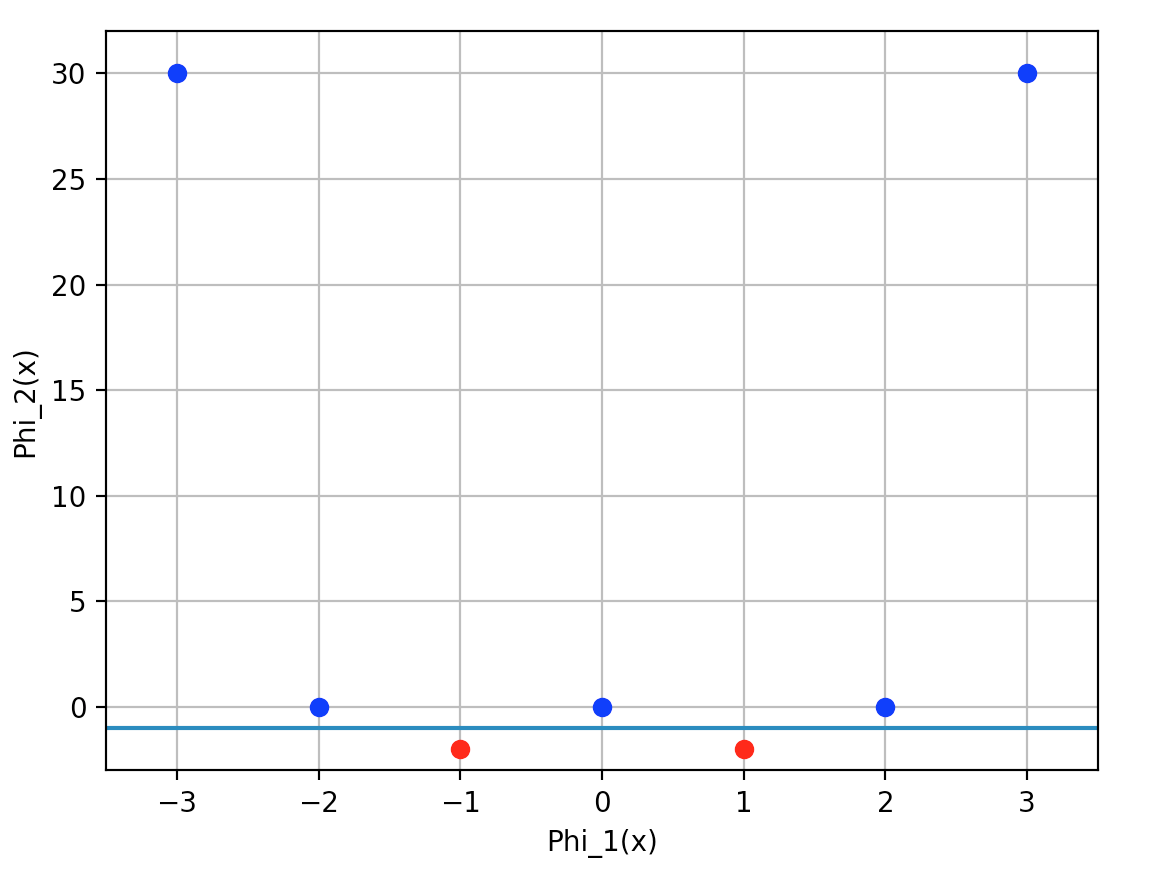
\includegraphics[scale=0.2]{1_1.png} \hfill
\includegraphics[scale=0.2]{1_05.png}\hfill
\includegraphics[scale=0.2]{1_0.png} \hfill\null

As intuition would suggest, a smaller eta leads to a slower, smoother convergence. This is because the step size during each iteration of the gradient descent is smaller. When eta is larger, at about $0.1$, the loss jumps sporadically during the iterations likely because we are overshooting the optimum and we are oscillating back and forth. However, there is a tradeoff, because a larger eta leads to faster convergence. In fact, with eta equal to $0.1$ and a lambda of $0$, my model was able to generate much smaller loss after $3000$ epochs compared with when I had a lambda of $0$ and a smaller eta.

As we would expect, having the regularization parameter, lambda, causes the minimum possible loss to be higher than if we had no regularization constraint. This is because turning off the regularization constraint allows our parameters to move freely and fit the data to the best ability given the design constraints of the model (in this case, linear boundaries). Also, I observed that with the regularization constraint, the gradient descent converged faster, which makes sense, because the loss cannot be minimized as much so we achieve our optimal loss sooner.

Ultimately, taking all these factors into consideration, I chose to use an eta of $0.05$ and a lambda of $0$. This allowed for the optimization to converge quickly and fit the data fairly well, as shown by plotting the loss:

\begin{center}
    \includegraphics[scale=0.5]{05_0.png}
\end{center}

It could be argued that the model does not converge smooth enough with these parameters (so we may be overshooting an optima). More epochs and a smaller eta would solve this. However, keeping my epochs at a reasonable level, I thought $0.05$ struck a good balance between speedy convergence rate and smooth descent. Additionally, I thought using $0$ as the value for lambda was a reasonable choice because the model seems to not overfit too much once the regularization conditions are removed (this is the reason we would keep lambda).


\item 
With shared covariance, the Gaussian generative model produced a negative log likelihood of $116.394$ while with separate covariance matrices for each class, it produced a negative log likelihood of $63.970$. Since negative log likelihood is our loss function (it assigns a penalty to any point with class $k$ which is assigned a probability of having class $C_k$ of less than $1$), we see that the negative log likelihoods confirm that the separate covariance Gaussian model is able to fit the data better than the shared covariance model.

\item 
For a star with magnitude 6 and temperature 2, my separate covariance Gaussian model predicts class 0 (Dwarf type) while the shared covariance Gaussian model and the logistic regression model both predict class 1 (Giant type). As we can see, the linear classifiers predict differently than the separate covariance Gaussian model (which has quadratic boundaries). This seems to point towards the separate covariance Gaussian model being more trustworthy since this new data point is far off of the line where the other Giant data points occur, and there are more Dwarf data points and they are more dispersed. Hence, from intuition, it seems that guessing Dwarf for this new star is reasonable. We see that the separate covariance Gaussian model is able to take these facts (number of data points and spread of data over a non-linearly separable area) into account more than the other models. 

However, I do have reservations about fully trusting this model, because a point could be fairly close the rest of the Giant stars but it would be predicted Dwarf, so perhaps this model is overfitting. More data would help!

\end{enumerate}

\newpage
\begin{itemize}
    \item Name: Zachary Dietz
    \item Email: zachdietz1@gmail.com
    \item Collaborators: Theo Walker, Ian Leifer
    \item Approximately how long did this homework take you to complete (in hours): 15
\end{itemize}
\end{document}